%% Fig. 1 is anchored BEFORE the heading (2026-09-13): a two-column float encountered after
%% the page's first column has started is deferred a full page, which cascaded into the
%% page budget when section I grew by three lines.
%% Source: figures-hand/pipeline.drawio -> pipeline.pdf (draw.io desktop, `-x -f pdf --crop`).
\begin{figure*}[t]
  \centering
  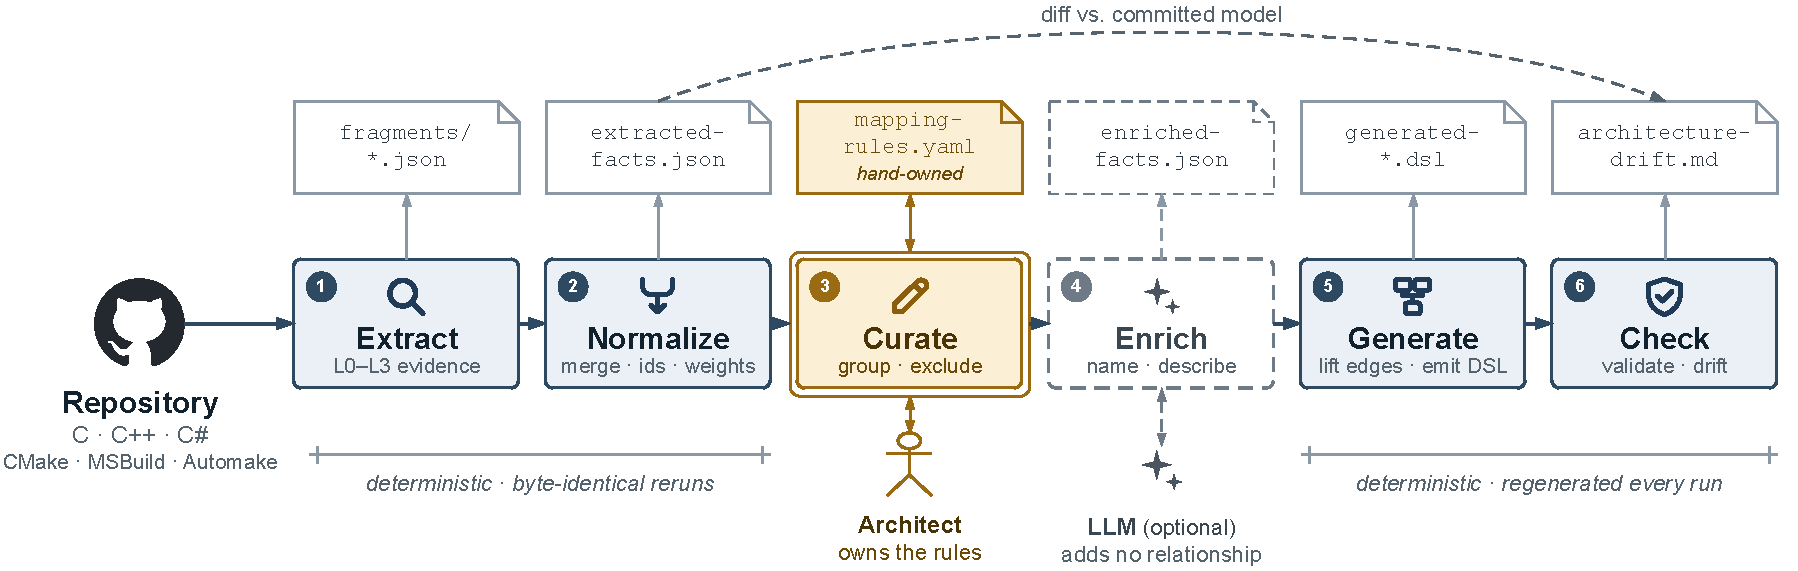
\includegraphics[width=0.9\textwidth]{figures-hand/pipeline.pdf}
  \caption{The pipeline. Blue stages are deterministic and regenerate byte-identically; the one
  human gate is stage~3, driven by the hand-owned mapping-rules file (amber, double border); the
  optional LLM stage (dashed) may only name and describe elements the evidence already contains,
  never add, remove, or move a relationship. Each stage writes the artifact above it; stage~6
  validates the model, checks the layering rules, and diffs freshly extracted facts against the
  committed model.}
  \label{fig:pipeline}
\end{figure*}
\section{Approach}
\label{sec:approach}

%% Revised 2026-08-30 against the GPT-5.6-Sol review and tightened for the page budget: module
%% (development) view scoped (6.1); "source of truth" -> primary evidence (A.2); L0--L3 (A.1);
%% LLM stage one paragraph, tested invariants stated here (4.6/A.7). Design constants are
%% literals on purpose. 2026-09-13 shortening pass (response plan §13, M6): the per-idiom extractor
%% detail added for the second review's point 5 keeps its substance (evaluated vs. static, what
%% each misses) and sends the target-type / alias / imported / partial handling and the generated
%% bash model figure (owner decision) to the TR.
%% 2026-09-13 readability pass: long sentences split, §III.A split into two paragraphs; no content change.


\tool{} turns a C/C++ or C\#\ repository into a governed model of its \emph{module view}: the
development-time decomposition into build targets and projects, and the compile-time dependencies
between them (link, include, symbol, and project references). It is rendered in the C4
notation~\cite{brown2026c4} of the Structurizr DSL~\cite{structurizrdsl}, the notation architects
keep. Using C4's container level for build units is a deliberate adaptation (a static library is
not a deployable unit): Structurizr's styles, drill-down, and tooling attach to that level. We
claim no runtime or deployment semantics.
Figure~\ref{fig:pipeline} shows the six stages. Three invariants shape every design decision: the
build graph is the primary structural evidence, which source-level evidence refines but never
replaces (\S\ref{sec:evidence}); a language model may name and describe elements but cannot add,
remove, or move a relationship (\S\ref{sec:enrich}); and the same inputs regenerate the same bytes
(\S\ref{sec:generate}). The first is a claim the study tests; the other two are held by tests on
every change.
% (a provider that invents a relationship is rejected; two runs must be byte-identical).

\subsection{Evidence extraction: build graph first}
\label{sec:evidence}

We distinguish evaluated from static extraction. For CMake the pipeline configures the project
once (Ninja generator) and reads CMake's File API codemodel of that configured tree: targets of
every type and the link dependencies as CMake evaluated them, generator expressions and conditions
included. For .NET the L0 layer is a static parse of \texttt{.sln} and \texttt{.csproj} files that
takes every \texttt{<ProjectReference>} regardless of MSBuild conditions and follows no import;
the Roslyn layer then loads the solution, an evaluated view. MSBuild C++ projects and automake or
hand-written \texttt{Makefile.in} are parsed statically: imports, property expansion, and
conditionals are not evaluated, so a conditional reference is over-approximated and one reachable
only through an import is missed (per-idiom detail and the graphviz cross-check of CMake edges:
\trExtract{}).

These declared dependencies form evidence layer L0; package references form L1; L2 adds the
\texttt{\#include} graph (Doxygen XML or \texttt{clang-scan-deps}) and Roslyn symbol references;
L3 (P/Invoke interop, deployment descriptors) is not evaluated here. Every extractor writes an
independent JSON fragment and degrades gracefully: without its toolchain it records a coverage
warning and an empty fragment. Per-layer coverage travels with the facts; its L0 denominator is
the first-party target set. A few \emph{refinement} extractors add no structure, only tags from
conventions the source declares (\texttt{.csproj} SDK role, OrchardCore module category, plugin
naming) for curation to group on. Declared dependencies are evidence, not truth (test, packaging,
and obsolete relations; missed runtime coupling), so curation excludes test and vendored targets
and the check stage reports a declared dependency no source file exercises.

\subsection{The fact model}
\label{sec:factmodel}

Normalization merges all fragments into one plain-JSON \emph{architecture fact model}, the
schema-validated contract between the extractors and any generator. Elements carry
content-independent identifiers (CMake target identity, project path), never a display name, so
a rename leaves identity intact and a move is pinned with an explicit alias. Evidence lists
citing the literal build-file
line, include, or symbol are concatenated and de-duplicated, and every derived quantity is
recomputed from the merged evidence. \emph{Weight}, the edge intensity the threshold of
\S\ref{sec:curate} reads, is a deterministic sum over that evidence, its constants pinned in one
module: 5 per declared link or project reference, 1 per package
reference, an include item's file count capped at 10 so one chatty header cannot dominate, a
symbol-use item's count, and 5 per P/Invoke. \emph{Confidence} is computed orthogonally (low for
a declared link no source exercises). Every edge with L0 evidence is marked \emph{declared}, no
relationship exists without evidence, all lists are canonically ordered, and a
provenance-stripped hash of the model is the idempotency and drift key.

\subsection{Curation: rules as code behind a human gate}
\label{sec:curate}

A dependency graph is the wrong altitude for an architecture diagram, so a curation step maps many
build targets onto fewer containers through a hand-reviewed \texttt{mapping-rules.yaml} in a
propose--review--lock loop. \cli~\texttt{propose} drafts rules from explainable heuristics
(layout, namespace roots, target-name patterns, edge weight, the convention tags above), and the
architect accepts or edits them in the YAML or a tree editor. Once committed, every run is
deterministic until a target appears that no rule covers; it is rendered as its own container
tagged \texttt{needs-curation}, never guessed. Rules group members by identifier, path
glob, or tag; exclude test, generated, and vendored targets; pin names; and set the significance
threshold (default 3) for non-declared edges only. A declared dependency is never dropped by
weight, only by explicit exclusion. The curator chooses the boxes; the evidence draws the arrows.

\subsection{Enrichment: language, not structure}
\label{sec:enrich}

The LLM stage is off by default and never runs in CI; the evaluated technique is the deterministic
one. Its input is the curated fact model after a redaction pass and a field whitelist:
identifiers, types, top dependencies, and documentation snippets of at most 280 characters, never
a source file. Its output is validated against a JSON schema and a referential-integrity check
that rejects any element or relationship the facts do not already contain, so its structural
footprint is zero by construction.

\subsection{Generation and governance}
\label{sec:generate}

The generator lifts target-to-target edges to container-to-container edges, merging parallel
and dropping intra-container ones, and emits two machine-owned DSL fragments that the
hand-owned \texttt{workspace.dsl} includes. Views, styles, and saved layout are scaffolded once,
and stable DSL identifiers let Structurizr re-attach saved positions after a regeneration (one
generated model with its evidence traced: \trExtract{}). The check stage diffs freshly extracted facts against the committed model and reports new and
vanished targets and edges, suspected renames, declared-but-unused dependencies, and violations of
forbidden container-to-container edges from a layering-rules file. Three stopping rules keep it
from crying wolf. A disappearance is drift only if the evidence layer that produced it was
extracted in both runs, otherwise a labelled coverage gap. Below 80\,\% first-party L0 coverage,
or with no first-party target extracted at all, the report is advisory and stops gating. A layering check over degraded evidence answers \texttt{UNVERIFIED} rather than passing.
Drift is always a report, never an automatic edit.
